\documentclass[conference]{IEEEtran}
\IEEEoverridecommandlockouts
% The preceding line is only needed to identify funding in the first footnote. If that is unneeded, please comment it out.
\usepackage{cite}
\usepackage{amsmath,amssymb,amsfonts}
\usepackage{algorithmic}
\usepackage{graphicx}
\usepackage{textcomp}
\usepackage{xcolor}
\def\BibTeX{{\rm B\kern-.05em{\sc i\kern-.025em b}\kern-.08em
    T\kern-.1667em\lower.7ex\hbox{E}\kern-.125emX}}
\begin{document}

\title{Analyse and data mining of a chromatograph during drilling operations}

\author{\IEEEauthorblockN{1\textsuperscript{st} Toma Becea}
    \IEEEauthorblockA{\textit{Automation and Computer Science Faculty} \\
    \textit{Technical University of Cluj-Napoca}\\
            Cluj-Napoca, Romania \\
            tomabecea@pm.me}
    \and
    \IEEEauthorblockN{2\textsuperscript{nd} Honoriu Vălean}
    \IEEEauthorblockA{\textit{Automation and Computer Science Faculty} \\
    \textit{Technical University of Cluj-Napoca}\\
            Cluj-Napoca, Romania \\
            Honoriu.Valean@aut.utcluj.ro}
}

\maketitle

\begin{abstract}
    Chromatograph analyses need a great attention to the way results are generated and how they are calibrated.
    At the same time the construction and maintenance need to be simple and quick such that any operation which
    needs to be made on a chromatograph doesn't stop the entire drilling crew.
\end{abstract}

\begin{IEEEkeywords}
chromatography, geology, mud-logging
\end{IEEEkeywords}

\section{Introduction}
    During drilling operations, while seeking gas or oil, certain gas analyses must be taken.
    Those analyses are performed by a special device called chromatograph. 
    Present paper presents a novel way of generating the mathematical model of a chromatograph during its construction
    and then using this model to ensure the results accuracy.
\section{chromatograph}

\subsection{Chromatography concepts}

    Gas chromatography means to separate components such that they can be analyzed independently. To achive this a
    separation column is used. A probe of gas, taken from drilling installation, is pushed through the column which
    means that all components enter into it at the same time. The column is filled with carefully choosen particles,
    whose type and size are competitive commercial advantages (and because this is not the object of the current paper,
    their details will not be disclosed). The probe is pushed through the column using a bearing gas, usually hydrogen.
    The probe has to make its way through the column's particles and because of the friction between them different
    components will have different speeds with which they advance. Thus, the components are reaching the end of the 
    column at different times. The time which is needed for a component to traverse the column is called retention time.
    Figure \ref{fig:column} contains a representation of a column and how two components, A and B, enter into the column at the same
    time but they exit at different times.
    
    During the usual drilling operations geologist engineers are interested in certain components so that they can analyze
    and predict the behavior of the gas or petrol reservoir. Those components are: methane (C1), ethane (C2), propane (C3),
    n-butane (nC4), isobutane (iC4), neopentane (nC5), isopentane (iC5). The sum of all those components yields a number
    called theoretical total gas. The probe is also analysed as a whole to find out the total gas. The ratio of those two
    numbers is of paramount importance.
    
    Among the details which can be find out using the analyses of those components are the quality of the gas or petrol
    which is in the reservoir, the proximity of the reservoir or certain predictors important for drilling engineers, for
    example, the danger of the entire reservoir to erupt.

    \begin{figure}
        \centering
        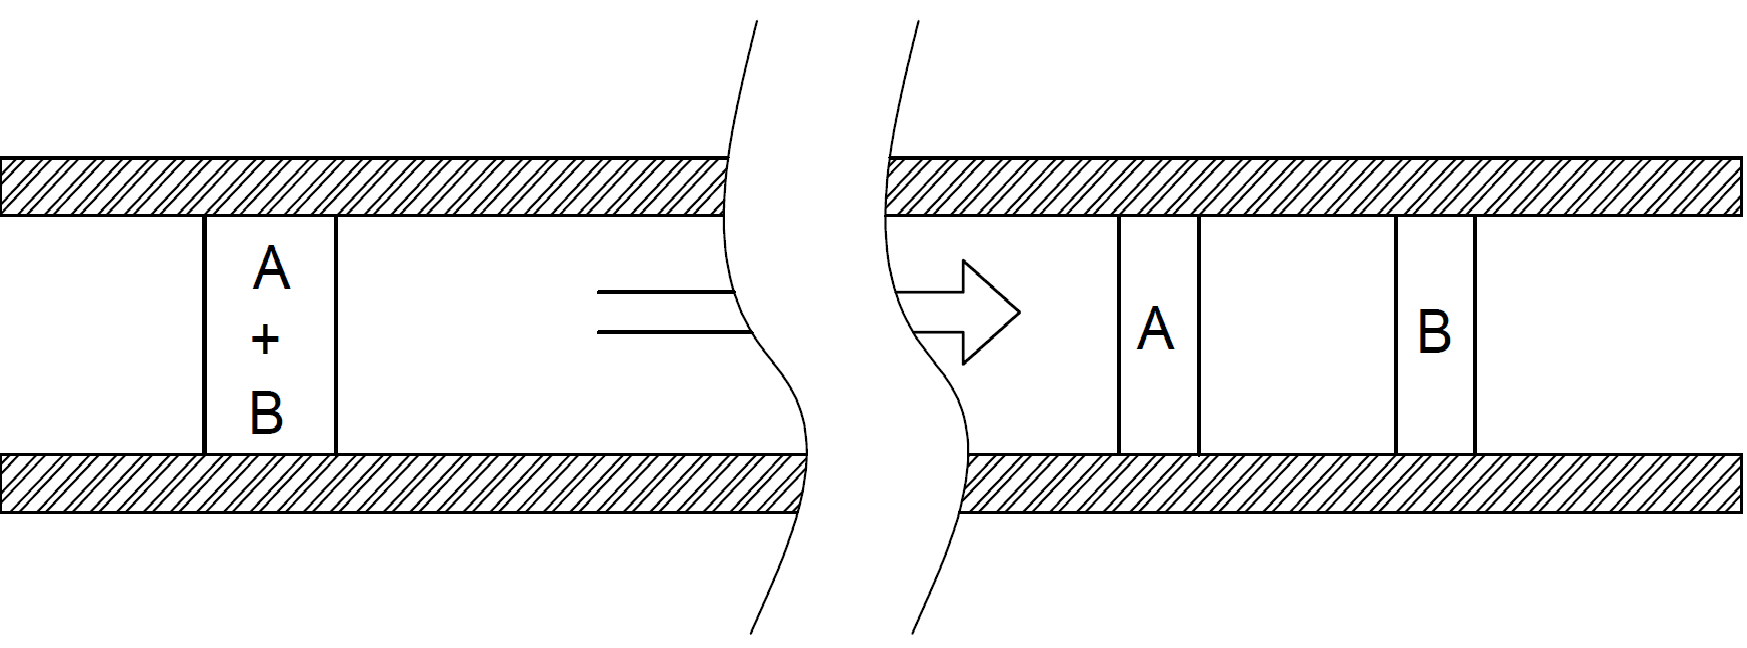
\includegraphics[width=0.5\textwidth]{column.png}
        \caption{Gas separation column}
        \label{fig:column}
    \end{figure}

\subsection{Flame Ionisation Detector}

    The components are slowly (or fast, depending on the performance of the chromatograph) pouring out of the column
    into a detector called Flame Ionisation Detector or FID. Its role is to transform over the analyses time the quantity
    of each component into voltage. This voltage is read by ADC boards and transmitted to a computer for further calculations.
    Figure \ref{fig:fid} shows the schematics of such a FID. Item 1 represents the separation column, item 2 represents suplimentary
    gas supply, 3 represents hydrogen supply, 4 represents the lighter, 5 represents the collector electrode, 6 is the
    polarizing electrode, 7 is the burner and 8 is the air supply.

    \begin{figure}
        \centering
        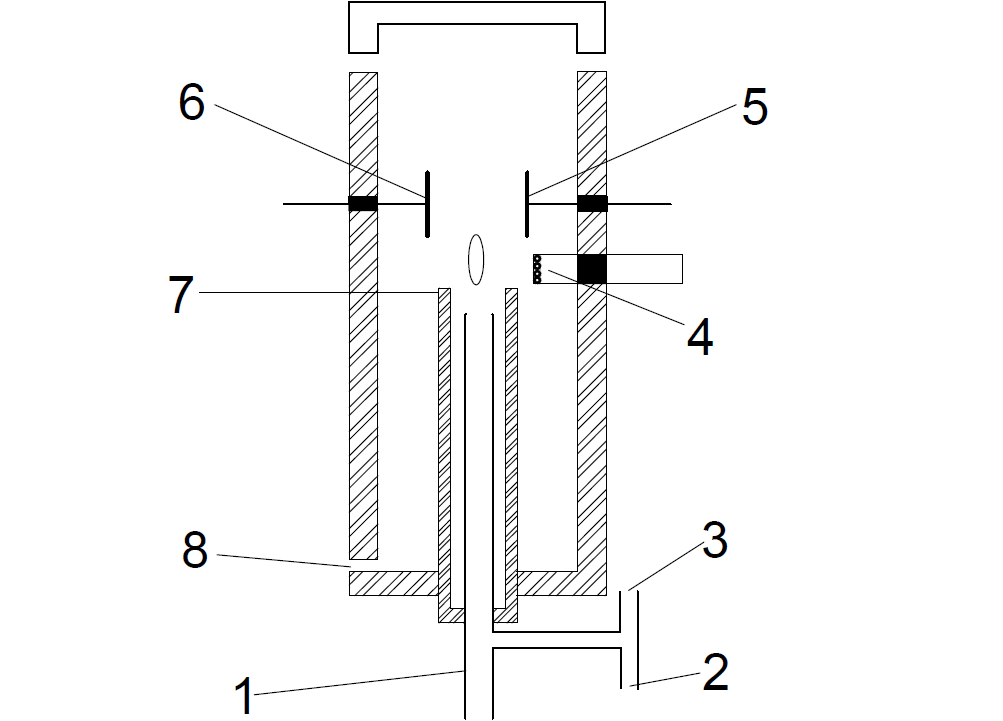
\includegraphics[width=0.5\textwidth]{fid.png}
        \caption{Flame Ionisation Detector}
        \label{fig:fid}
    \end{figure}

\subsection{Construction}
    
    Following description will be a brief one and it focuses only on what is important for this paper. The construction of a 
    chromatograph implies certain components to be glued together. We have already seen the separation columns. Those are 
    two or three wired through special designed pneumatics components. Then there might be two or three FIDs where the
    output of the columns is going. The entire process also needs a source of compressed air and a source of hydrogen. For
    easier manipulation the front panel may contain analog pressure indicators and few knobs for pressure and hydrogen
    regulation.

    The FIDs have two electrodes which are wired to a ADC converter through a special interface that has the output between
    0 Volts and 10 Volts. The ADC converts this data into a digital format and sends it to a computer over a USB connection.

    Following the mechanical construction of such a chromatograph the engineer who built it needs to calibrate it. For this
    a calibrating gas is used and injected via a face mounted pneumatic orifice. The chromatograph will analyze the gase received
    from this input, rather than the gas received from the usual output, i.e. site drilling rig.
    
    Therefore, an easy approach should be considered on delivering a chromatograph with ready-to-use software.
    
\subsection{Maintenance}

    A drilling site is filled with dust, the temperatures might drop below freezing for extended periods of time, the mud is
    a constant and the mechanical load during transport from one site to another is a burden. Then there always might be extended
    periods with no activity. 

    Therefore, the chromatograph must be easy to setup again, easy to start and easy to calibrate again because in time its 
    FID characteristic tend to skew.

    There are also periodic calibration of the chromatograph for better results and for verifying that certain results, which
    might seem odd at first, are actually real.

    Both the construction side of a chromatograph and its maintenance makes the designer of this device to consciously design
    it for those situations.

    \begin{figure}
        \centering
        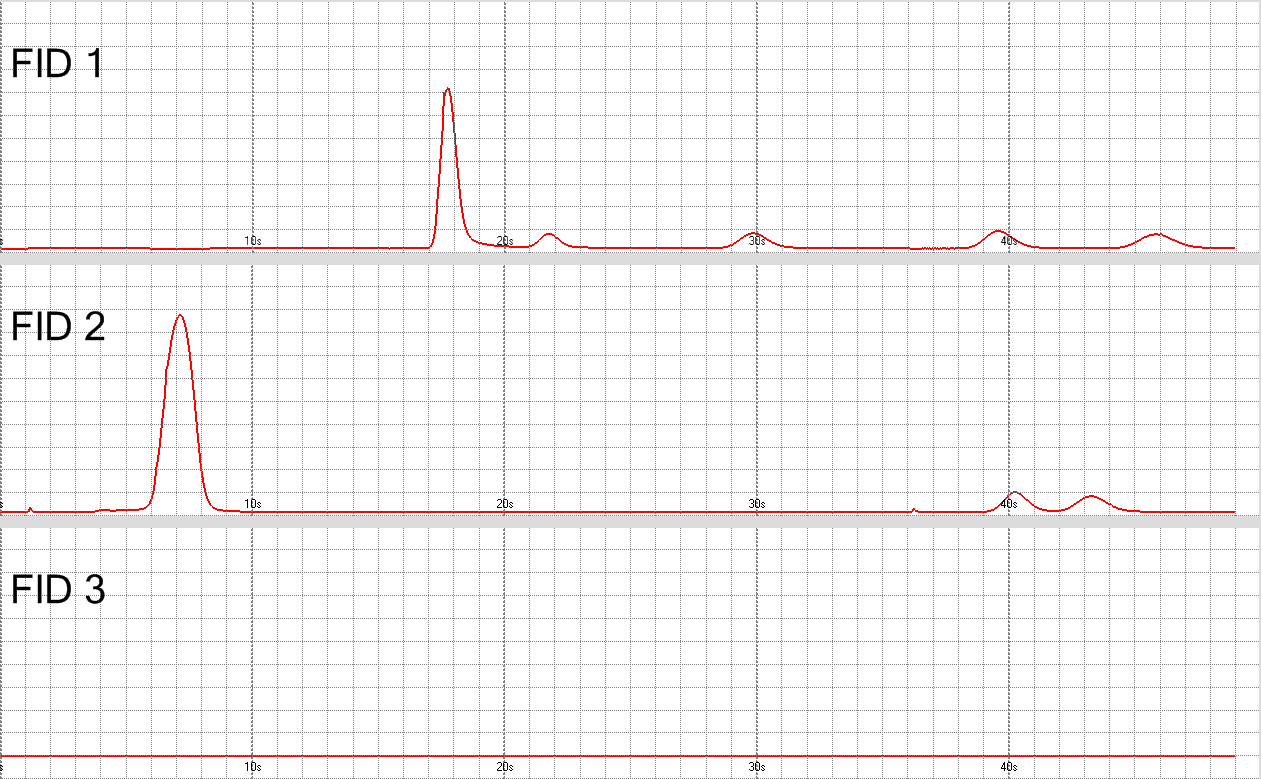
\includegraphics[width=0.5\textwidth]{fidgraph.png}
        \caption{FID Graph}
        \label{fig:fidgraph}
    \end{figure}

\section{Mathematical model}

    The mathematical model is so simple, one could wonder if it works at all: it's based on the least squares equation.
    From figure \ref{fig:fidgraph} it can be seen that during one minute of analyses the first two FIDs have some components present.
    Using different rules for establishing a baseline the area of each component (each "hill") is computed. This area is 
    proportional with the amount of the component from the last probe analysed. The engineer who builds the chromatograph and then
    the engineer who maintain it will introduce, in consecutive analyses, different gases with a precisely known composition, using
    different concentrations. Thus, a series of analyses will be made, knowing for each one the calibrating gas composition and the
    results. A look tabel is born from this operation.

    During normal operations the look up tabel will be used to analyze gases from drilling site. To be able to give results for any
    given concentration, for any given component, an interpolation is needed between two known points, using first two points or
    using last two points. This kind of interpolation is very similar to an average between two numbers. Equation \ref{eq:average}
    represents such an average: \(K_n\) and \(K_{n+1}\) are numerical integrations results and  \(C_n\) and \(C_{n+1}\) are
    corresponding component's concentrations from the lookup table. \(R\) will be the result of the current analyze.    

    \begin{equation}
        R = \frac{C_n + C_{n+1}}{K_n + K_{n+1}}, K_{n} \leq R \leq K_{n+1}
        \label{eq:average}
    \end{equation}

    Another method for obtaining results using the data from the lookup table is to use the least squares method. Equation \ref{eq:leastSquares}
    shows the gist of this method. \(x_{1}\) through \(x_{n}\) are the known concentrations from calibration operation. \(y\) terms are
    the numerical integration results for a component, for each concentration. \(b\) terms are the coefficients which are found by 
    solving the equation \ref{eq:leastSquares}. \(b\) terms will form a polynom which will be used during normal analyze mode to computed
    the real concentration of a component from a probe taken from the drilling site.

    \begin{equation}
        \begin{bmatrix}
             x_0 \\ \vdots \\ x_{n} 
         \end{bmatrix}
             =
         \begin{pmatrix}
            y_{00} & \hdots & y_{0(m-1)} & y_{0m}\\
            \vdots & & \vdots & \vdots \\
            y_{n0} & \hdots & y_{n(m-1)} & y_{nm}
            \end{pmatrix}
            \times
            \begin{pmatrix}
            b_0 \\ \vdots \\ b_m
        \end{pmatrix}
        \label{eq:leastSquares}
    \end{equation}


\begin{thebibliography}{00}
\bibitem{b1} G. Becea, ``First steps in chromatography'' Internal document of S.C. Daflog S.R.L., 2007.
\bibitem{b2} T. Beu ``Numerical analyses in Turbo Pascal'', 1992.
\bibitem{b3} I. Ciucanu, ``Gas chromatography with capilar columns'' 1990.
\end{thebibliography}
\vspace{12pt}

\end{document}
